\documentclass[border=0pt,10pt]{standalone}
\usepackage[T1]{fontenc}
\usepackage{lmodern}
\usepackage{pgfplots}
\pgfplotsset{compat=1.17}
\usepgfplotslibrary{groupplots}
\usepackage{xcolor}
\definecolor{oi-blue}{HTML}{0072B2}
\definecolor{oi-vermillion}{HTML}{D55E00}
\definecolor{oi-green}{HTML}{009E73}
\definecolor{oi-purple}{HTML}{CC79A7}
\definecolor{oi-black}{HTML}{000000}
% semantic_sha256: bd2a953e6fdeba82f892112e77e569b479863bd0d1672a21f119ca1f80c333bc
\begin{document}
\begin{minipage}{181.86mm}
\centering
{\bfseries\fontsize{10}{12}\selectfont PP-U-SG | D2 | source\_fit}\\[2mm]
{\fontsize{8}{10}\selectfont planned=66, monitored=63, missing-history=3, status=partial\_history\_coverage}\\[3mm]
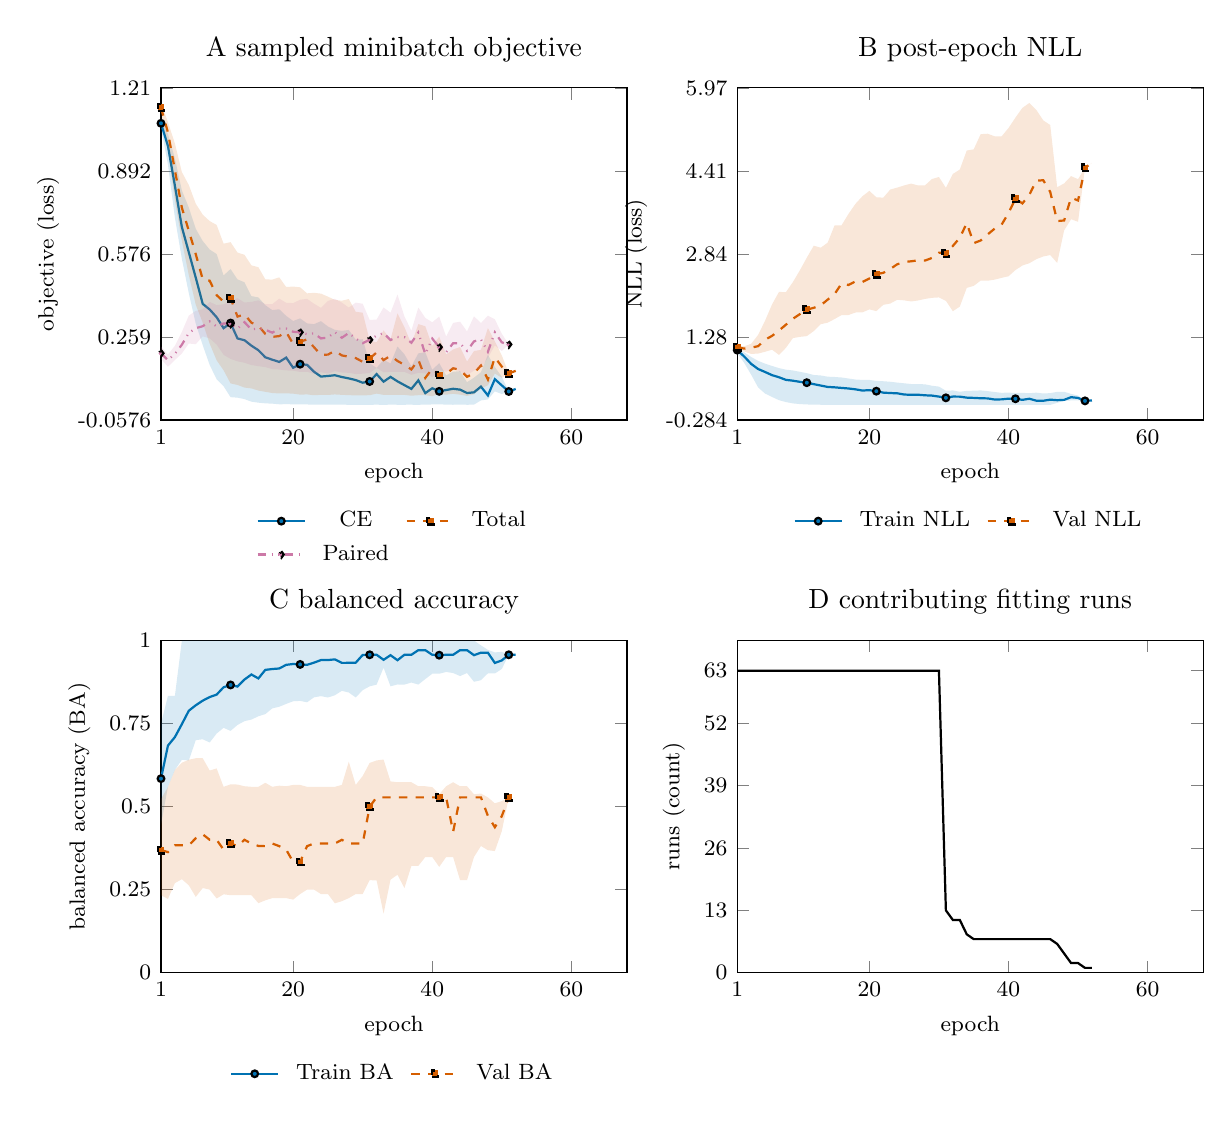
\begin{tikzpicture}
\begin{groupplot}[group style={group size=2 by 2, horizontal sep=14mm, vertical sep=28mm}]
\nextgroupplot[width=75mm, height=58mm, title={A sampled minibatch objective}, xlabel={epoch}, ylabel={objective (loss)}, xmin=1, xmax=68, xtick={1,20,40,60}, ymin=-0.057554432451725007, ymax=1.208643081486225, ytick={-0.057554432451725007,0.25899494603276252,0.57554432451725002,0.89209370300173751,1.208643081486225}, yticklabels={-0.0576,0.259,0.576,0.892,1.21}, tick label style={font=\fontsize{8}{9}\selectfont, text=black}, label style={font=\fontsize{8}{9}\selectfont, text=black}, title style={font=\fontsize{10}{11}\selectfont, text=black}, legend style={at={(0.5,-0.24)},anchor=north,draw=none,fill=none,font=\fontsize{8}{9}\selectfont,row sep=1pt,column sep=4pt,legend columns=2}]
\addplot[fill=oi-blue,opacity=0.15,draw=none,forget plot] coordinates {(1,1.0559110939502716) (2,0.91612630188465116) (3,0.71392716169357295) (4,0.55689769983291626) (5,0.42564327418804171) (6,0.30937913954257967) (7,0.2277863584458828) (8,0.15243482291698457) (9,0.097748534381389612) (10,0.071276510879397389) (11,0.029608484264463188) (12,0.027731633838266136) (13,0.022262682905420661) (14,0.012447815435007215) (15,0.0086179302306845784) (16,0.0060600428609177467) (17,0.0048758941411506385) (18,0.0025250255828723313) (19,0.0027838682071887888) (20,0.0025389915535924956) (21,0.0018668333708774299) (22,0.0017526711511891336) (23,0.0012926500145113095) (24,0.0011972021486144513) (25,0.00094789900758769359) (26,0.0016519688433618285) (27,0.00088368097131024119) (28,0.00065404112683609128) (29,0.00070495754989678976) (30,0.0005835919131641276) (31,0.00066944649443030375) (32,0.00079016343806870282) (33,0.00061729591834591702) (34,0.00082074557103624108) (35,0.0007238663645694033) (36,0.00072449405270162974) (37,0.00078539180103689434) (38,0.00052735329081770037) (39,0.0012745486506901217) (40,0.0017917077377205715) (41,0.002553701199940406) (42,0.0010693678756069859) (43,0.00069952182529959823) (44,0.0016937974076427055) (45,0.00062309738241310701) (46,0.0011501254273753149) (47,0.017331005749838369) (48,0.020992241194471718) (49,0.051716761686839162) (50,0.041622955771163109) (51,0.051335785072296858) (52,0.060803130269050598) (52,0.060803130269050598) (51,0.051335785072296858) (50,0.10722799231298268) (49,0.14485027662012726) (48,0.190842430992052) (47,0.12466306588612497) (46,0.10414213687181473) (45,0.086642842367291459) (44,0.1287552757188678) (43,0.12645306661725048) (42,0.11291648373007775) (41,0.15934928804636003) (40,0.13378026112914088) (39,0.20052697584033016) (38,0.19664800837635996) (37,0.14715578928589823) (36,0.19312860742211344) (35,0.22256944924592975) (34,0.1579965589568019) (33,0.17274990305304527) (32,0.14122978784143925) (31,0.1589166209101677) (30,0.25046213865280154) (29,0.24890592768788344) (28,0.28578743413090724) (27,0.28259823471307766) (26,0.28638533130288124) (25,0.29901875555515295) (24,0.31938810423016561) (23,0.30788092687726026) (22,0.31094607487320902) (21,0.32982566654682161) (20,0.32007513418793676) (19,0.33944244086742409) (18,0.36468618065118791) (17,0.36147149503231052) (16,0.38003164082765595) (15,0.40995254665613184) (14,0.41489241570234303) (13,0.46759635806083683) (12,0.47863980084657676) (11,0.51803067922592161) (10,0.49370565712451936) (9,0.57534791529178619) (8,0.59244482964277267) (7,0.62491303384304053) (6,0.6714399635791779) (5,0.75215109288692472) (4,0.81800474226474762) (3,0.94002310335636141) (2,1.0331793665885927) (1,1.087944358587265)};
\addplot[color=oi-blue, mark=*, mark options={draw=black}, mark repeat=10, mark size=1.2pt, solid, line width=0.8pt] coordinates {(1,1.0735045671463013) (2,0.9872078001499176) (3,0.83543166518211365) (4,0.67808109521865845) (5,0.58186913281679153) (6,0.48499427735805511) (7,0.38528846204280853) (8,0.36384526640176773) (9,0.33433465659618378) (10,0.29266363382339478) (11,0.31219805777072906) (12,0.25352628156542778) (13,0.24673445895314217) (14,0.22592572495341301) (15,0.20865423977375031) (16,0.18164901435375214) (17,0.17247133329510689) (18,0.16398210451006889) (19,0.18040563352406025) (20,0.14160821121186018) (21,0.1554270051419735) (22,0.15283050388097763) (23,0.12657447531819344) (24,0.1081104464828968) (25,0.11049081198871136) (26,0.1132368054240942) (27,0.10646883398294449) (28,0.1011100891046226) (29,0.094817698933184147) (30,0.08475218154489994) (31,0.089393731206655502) (32,0.11749703623354435) (33,0.088711800519376993) (34,0.1069059120491147) (35,0.089923445135354996) (36,0.075432037934660912) (37,0.061255702748894691) (38,0.093632492236793041) (39,0.045071287080645561) (40,0.063629920594394207) (41,0.051815883256494999) (42,0.056990764103829861) (43,0.061577661661431193) (44,0.058427200652658939) (45,0.045493758632801473) (46,0.048092205193825066) (47,0.069879124639555812) (48,0.03625936433672905) (49,0.098283519153483212) (50,0.074425474042072892) (51,0.051335785072296858) (52,0.060803130269050598)};
\addlegendentry{CE}
\addplot[fill=oi-vermillion,opacity=0.15,draw=none,forget plot] coordinates {(1,1.1140403509140016) (2,0.97109899520874021) (3,0.77899411618709569) (4,0.62529561221599583) (5,0.49488540291786193) (6,0.38196536302566531) (7,0.31340039074420928) (8,0.23364674597978591) (9,0.17023954167962074) (10,0.1321480765938759) (11,0.082115637511014944) (12,0.076146593876183027) (13,0.066229063831269738) (14,0.063025072962045667) (15,0.054866028577089311) (16,0.05002656280994415) (17,0.045454894006252286) (18,0.043747124541550872) (19,0.044169032759964463) (20,0.043115081265568733) (21,0.039289736002683637) (22,0.040126308798789978) (23,0.036958115175366402) (24,0.038541400898247959) (25,0.038050573319196701) (26,0.040065582655370233) (27,0.038424894120544194) (28,0.037371765635907647) (29,0.036271074227988719) (30,0.036618958599865435) (31,0.037141619622707366) (32,0.043138883542269468) (33,0.038365679793059826) (34,0.038622330222278831) (35,0.038603505957871674) (36,0.038321764580905436) (37,0.035234621353447439) (38,0.037172963097691539) (39,0.037217010371387006) (40,0.03348913677036762) (41,0.041838035732507703) (42,0.03907612767070532) (43,0.042461522482335569) (44,0.039201096072793006) (45,0.034449340682476758) (46,0.040469132177531716) (47,0.062466562958434224) (48,0.074946602620184419) (49,0.1198224239051342) (50,0.10339209828525782) (51,0.12056275643408298) (52,0.12980069033801556) (52,0.12980069033801556) (51,0.12056275643408298) (50,0.18861918691545726) (49,0.2427859865128994) (48,0.29294238053262239) (47,0.20987840183079243) (46,0.20552685074508192) (45,0.16561176627874374) (44,0.22076185755431654) (43,0.21139873042702678) (42,0.19254466220736505) (41,0.26038732975721363) (40,0.22491594552993777) (39,0.30005260780453685) (38,0.30805995017290116) (37,0.23212864845991135) (36,0.29657922908663747) (35,0.34877442643046386) (34,0.24988464936614035) (33,0.2842768207192421) (32,0.23883929848670959) (31,0.24508184418082238) (30,0.35174431204795836) (29,0.35518636852502822) (28,0.40366240292787559) (27,0.39736941307783147) (26,0.40034729242324829) (25,0.41281553059816362) (24,0.42433925271034256) (23,0.42739175856113454) (22,0.42543014436960225) (21,0.44844058603048331) (20,0.45122090280055999) (19,0.44953860640525822) (18,0.48640454262495048) (17,0.47779511809349062) (16,0.47872903794050226) (15,0.52504584044218072) (14,0.53211048841476449) (13,0.57241427004337309) (12,0.58074235916137695) (11,0.62052125632762911) (10,0.61475956439971924) (9,0.68608193844556808) (8,0.70091647207736973) (7,0.72531504929065704) (6,0.76705558896064763) (5,0.83827161192893984) (4,0.88763264119625096) (3,0.99648519456386575) (2,1.0778143584728241) (1,1.1510886490345)};
\addplot[color=oi-vermillion, mark=square*, mark options={draw=black}, mark repeat=10, mark size=1.2pt, dashed, line width=0.8pt] coordinates {(1,1.1334004700183868) (2,1.0386315882205963) (3,0.89478762447834015) (4,0.75183118879795074) (5,0.66372571885585785) (6,0.57469214498996735) (7,0.4786158874630928) (8,0.47367001324892044) (9,0.41851283609867096) (10,0.39370523393154144) (11,0.40724775940179825) (12,0.33673282712697983) (13,0.34509886801242828) (14,0.31367423385381699) (15,0.30182818323373795) (16,0.27083730325102806) (17,0.25951411575078964) (18,0.26248686388134956) (19,0.27794007956981659) (20,0.23269851133227348) (21,0.24022875726222992) (22,0.25010037794709206) (23,0.22001281753182411) (24,0.19078903272747993) (25,0.19192545115947723) (26,0.2062743566930294) (27,0.18877239339053631) (28,0.18391665071249008) (29,0.17858686484396458) (30,0.16437403485178947) (31,0.17675260454416275) (32,0.20014037936925888) (33,0.17093178629875183) (34,0.187675841152668) (35,0.16766723617911339) (36,0.15295310318470001) (37,0.13531605713069439) (38,0.17218393832445145) (39,0.10314352065324783) (40,0.13805318251252174) (41,0.11428334563970566) (42,0.1186944991350174) (43,0.13985789380967617) (44,0.13403656333684921) (45,0.10737416986376047) (46,0.12077020294964314) (47,0.1504030404612422) (48,0.096897737123072147) (49,0.1813042052090168) (50,0.14600564260035753) (51,0.12056275643408298) (52,0.12980069033801556)};
\addlegendentry{Total}
\addplot[fill=oi-purple,opacity=0.15,draw=none,forget plot] coordinates {(1,0.17521744668483735) (2,0.14554248116910457) (3,0.17131851315498353) (4,0.19616676568984986) (5,0.23407884761691095) (6,0.23169035464525223) (7,0.26141102910041808) (8,0.25372503399848939) (9,0.23023085817694663) (10,0.19095649346709251) (11,0.17530378624796866) (12,0.16612654030323029) (13,0.16085623577237129) (14,0.15204197913408279) (15,0.14762389473617077) (16,0.14418631233274937) (17,0.13635375462472438) (18,0.1349111557006836) (19,0.13153887093067168) (20,0.13058139234781266) (21,0.12569293566048145) (22,0.12617115303874016) (23,0.11874967217445373) (24,0.12455828934907913) (25,0.11971214115619659) (26,0.1286263071000576) (27,0.12368124611675739) (28,0.12236669361591339) (29,0.11771347895264625) (30,0.11906646564602852) (31,0.12142888531088829) (32,0.14116239547729492) (33,0.12445785664021969) (34,0.12600527703762054) (35,0.12626546137034894) (36,0.12578361444175243) (37,0.11497169919312) (38,0.12230831831693649) (39,0.11980820149183273) (40,0.10565808936953544) (41,0.13248411118984221) (42,0.12668919451534749) (43,0.13920666314661503) (44,0.12632149830460548) (45,0.11315285675227642) (46,0.13106334991753102) (47,0.1407944867387414) (48,0.17945943213999271) (49,0.22701886072754859) (50,0.20589712746441363) (51,0.23075655847787857) (52,0.2299918532371521) (52,0.2299918532371521) (51,0.23075655847787857) (50,0.27130396552383901) (49,0.32645235434174535) (48,0.34033317714929584) (47,0.31198345497250557) (46,0.33794903010129934) (45,0.28024116903543472) (44,0.31732060909271248) (43,0.31277820393443106) (42,0.2606419533491135) (41,0.33679346740245819) (40,0.31504184305667876) (39,0.33175209090113644) (38,0.37137313187122345) (37,0.28324286490678785) (36,0.3371041484177113) (35,0.42068325132131579) (34,0.35139871761202812) (33,0.37175638973712921) (32,0.32536500692367554) (31,0.32403836548328402) (30,0.38574136197566988) (29,0.38994734436273576) (28,0.37119917124509816) (27,0.39007401168346412) (26,0.40462002307176598) (25,0.39647920131683351) (24,0.37020814120769502) (23,0.38585672676563265) (22,0.40441015958786014) (21,0.40093480050563818) (20,0.38824369162321093) (19,0.3894442692399025) (18,0.40531785339117055) (17,0.38428135961294174) (16,0.38422849923372271) (15,0.39865737110376359) (14,0.39302751272916797) (13,0.39053749889135358) (12,0.40714549124240879) (11,0.39750557392835623) (10,0.38377819210290914) (9,0.38071843981742859) (8,0.39299495667219164) (7,0.36497930735349654) (6,0.35856130719184881) (5,0.34073811471462251) (4,0.2782709851861) (3,0.22547338157892227) (2,0.19256962090730667) (1,0.22246895208954812)};
\addplot[color=oi-purple, mark=diamond*, mark options={draw=black}, mark repeat=10, mark size=1.2pt, dash dot dot, line width=0.8pt] coordinates {(1,0.19693645834922791) (2,0.17046190425753593) (3,0.19510291144251823) (4,0.22954598441720009) (5,0.27419695258140564) (6,0.29252062737941742) (7,0.30015234649181366) (8,0.31838050112128258) (9,0.29901979118585587) (10,0.31065522134304047) (11,0.3095681369304657) (12,0.29103365540504456) (13,0.31554115563631058) (14,0.28749975562095642) (15,0.29172266274690628) (16,0.28653954714536667) (17,0.27560841664671898) (18,0.2909424789249897) (19,0.29115796461701393) (20,0.27888604253530502) (21,0.27706130966544151) (22,0.26993958652019501) (23,0.27258478850126266) (24,0.25356505438685417) (25,0.2570418119430542) (26,0.27774571999907494) (27,0.25602395832538605) (28,0.27433352917432785) (29,0.25325422361493111) (30,0.23544799163937569) (31,0.2480851523578167) (32,0.26417006179690361) (33,0.27406659349799156) (34,0.2474902831017971) (35,0.25914597511291504) (36,0.25840355083346367) (37,0.23714259639382362) (38,0.27580778300762177) (39,0.19357409328222275) (40,0.25295150652527809) (41,0.22041168808937073) (42,0.20083359628915787) (43,0.23541032150387764) (44,0.23431119695305824) (45,0.20626802369952202) (46,0.24225998297333717) (47,0.250138059258461) (48,0.20261344499886036) (49,0.27673560753464699) (50,0.23860054649412632) (51,0.23075655847787857) (52,0.2299918532371521)};
\addlegendentry{Paired}
\nextgroupplot[width=75mm, height=58mm, title={B post-epoch NLL}, xlabel={epoch}, ylabel={NLL (loss)}, xmin=1, xmax=68, xtick={1,20,40,60}, ymin=-0.28430119507859269, ymax=5.9703250966504458, ytick={-0.28430119507859269,1.2793553778536668,2.8430119507859266,4.406668523718186,5.9703250966504458}, yticklabels={-0.284,1.28,2.84,4.41,5.97}, tick label style={font=\fontsize{8}{9}\selectfont, text=black}, label style={font=\fontsize{8}{9}\selectfont, text=black}, title style={font=\fontsize{10}{11}\selectfont, text=black}, legend style={at={(0.5,-0.24)},anchor=north,draw=none,fill=none,font=\fontsize{8}{9}\selectfont,row sep=1pt,column sep=4pt,legend columns=2}]
\addplot[fill=oi-blue,opacity=0.15,draw=none,forget plot] coordinates {(1,0.9783112020602065) (2,0.79222181633219402) (3,0.57053324383648485) (4,0.33064583896352723) (5,0.21448520203214536) (6,0.1508619987806204) (7,0.089822018206732177) (8,0.054031263718986908) (9,0.029150208227747141) (10,0.016259005700117016) (11,0.008981392806300257) (12,0.0050088836993085256) (13,0.0034625044555946886) (14,0.0024607329325893458) (15,0.0016330325966639613) (16,0.0011123900134359581) (17,0.00050888620092391331) (18,0.00049273388584775743) (19,0.00039932452834778994) (20,0.0002624663181197411) (21,0.00022659066518875481) (22,0.00017749599679203946) (23,0.00017706508775172392) (24,0.00014326447436181593) (25,0.00014611064279712721) (26,0.00015617076106629342) (27,0.00011513523781040154) (28,9.0046675717233156e-05) (29,8.2155378683826066e-05) (30,7.6429115370248331e-05) (31,7.9744223866446242e-05) (32,0.00011616253922323941) (33,7.8240312890087506e-05) (34,8.874631165408956e-05) (35,9.2137418015627987e-05) (36,7.8003518472512121e-05) (37,6.8028749070910992e-05) (38,6.0461695901099152e-05) (39,5.5378814655161083e-05) (40,5.5013014730233895e-05) (41,5.2076189274661544e-05) (42,5.0405531378283764e-05) (43,7.049268102381723e-05) (44,7.6263814283762148e-05) (45,5.5963527476167297e-05) (46,4.6522037014141351e-05) (47,0.039053403695994707) (48,0.079241546405677821) (49,0.084373241231470525) (50,0.087185154595148265) (51,0.076850388084201596) (52,0.084227568712131592) (52,0.084227568712131592) (51,0.076850388084201596) (50,0.17675454037488425) (49,0.207738898487586) (48,0.24782707742460469) (47,0.24626374117479657) (46,0.22200985566121412) (45,0.21604848988181574) (44,0.23158854153459668) (43,0.22020954077494218) (42,0.22768034511351934) (41,0.2237317464465646) (40,0.23288888078026446) (39,0.22779965010000083) (38,0.24376409887648934) (37,0.26041030140424593) (36,0.27357711080032132) (35,0.26797180378998348) (34,0.26485540403366697) (33,0.24800019685215849) (32,0.27334131665115219) (31,0.26681637477887549) (30,0.34501872974246628) (29,0.36176209059846787) (28,0.38854601546149803) (27,0.39195243442062294) (26,0.39384208824525357) (25,0.40758468561574973) (24,0.42088064821896548) (23,0.43656654327022887) (22,0.44619734003451422) (21,0.45318096004822117) (20,0.47084379557039457) (19,0.47120329525948024) (18,0.4786715448695199) (17,0.49761894620792968) (16,0.51665698922217307) (15,0.52639860893356194) (14,0.53223599472769179) (13,0.55498229031117474) (12,0.56410924660030015) (11,0.59841126467077721) (10,0.62376887487354038) (9,0.64970210107890036) (8,0.66382714849239743) (7,0.6934661431256619) (6,0.73442115166857391) (5,0.77696094517144587) (4,0.8300684097558787) (3,0.90352605008102349) (2,0.99092094071108971) (1,1.0669363734192718)};
\addplot[color=oi-blue, mark=*, mark options={draw=black}, mark repeat=10, mark size=1.2pt, solid, line width=0.8pt] coordinates {(1,1.0324837775352744) (2,0.91214612377427995) (3,0.77334114707798218) (4,0.67660722450310029) (5,0.6205536832654337) (6,0.56120776838789277) (7,0.52159944838141992) (8,0.47217319469299374) (9,0.45643179647413651) (10,0.43519845675301416) (11,0.41906691085736841) (12,0.39138378122816042) (13,0.36523132962377669) (14,0.3391588787573544) (15,0.33159432105214343) (16,0.32025233306192996) (17,0.30974911700851848) (18,0.29361297001581504) (19,0.27110133608630937) (20,0.27840852690275059) (21,0.25889226734956494) (22,0.23164324443958259) (23,0.22416054903109986) (24,0.21896596299455656) (25,0.19626842415407977) (26,0.19033650386146941) (27,0.1921632183171644) (28,0.1814850440464435) (29,0.1759460653811358) (30,0.1572344428742177) (31,0.13404411455707291) (32,0.15745305452903449) (33,0.15610470781040939) (34,0.13748698333168535) (35,0.13254436964390451) (36,0.12607371693445305) (37,0.12296083228447727) (38,0.10228928628589473) (39,0.10492546838682752) (40,0.11789320157981001) (41,0.11615010520485999) (42,0.095661940373411372) (43,0.11647808944459793) (44,0.080061781699426376) (45,0.078881754492145531) (46,0.099472201775036864) (47,0.089496954580252253) (48,0.095784342097734232) (49,0.14605606985952826) (50,0.13196984748501625) (51,0.076850388084201596) (52,0.084227568712131592)};
\addlegendentry{Train NLL}
\addplot[fill=oi-vermillion,opacity=0.15,draw=none,forget plot] coordinates {(1,1.0551175904210832) (2,1.0078891055471964) (3,0.96039377561013994) (4,0.9673706790569746) (5,1.0012919087771015) (6,1.0405714870799336) (7,0.94254454609615834) (8,1.0756712673415727) (9,1.2579831465064364) (10,1.2818606988972734) (11,1.2955887534991981) (12,1.3906461320705106) (13,1.5200383237064357) (14,1.5490476634457224) (15,1.6175942031514887) (16,1.6921214970958409) (17,1.6932990428050125) (18,1.7404804597624037) (19,1.7434829207573428) (20,1.7992993347635298) (21,1.7670041655346016) (22,1.8852220527383714) (23,1.9091451257636822) (24,1.9801903805266758) (25,1.9694704682489714) (26,1.9486907861959151) (27,1.9670291935833586) (28,1.9963527729417661) (29,2.016978635685267) (30,2.0246234882151022) (31,1.9603151885549619) (32,1.7637578938973162) (33,1.8520425631167545) (34,2.2044679233206521) (35,2.2414592833928522) (36,2.341987010384956) (37,2.338714970783025) (38,2.3592908177308112) (39,2.3929315018657364) (40,2.4225783425906044) (41,2.5391683426353127) (42,2.6255242997889039) (43,2.6685310389573433) (44,2.7445459818252038) (45,2.7955840821628262) (46,2.8226353992588904) (47,2.67444170799667) (48,3.2860766231219958) (49,3.497036404005275) (50,3.4487078243417724) (51,4.4643548870553662) (52,4.5584824315365866) (52,4.5584824315365866) (51,4.4643548870553662) (50,4.2513338824557279) (49,4.3088776087236536) (48,4.1715486833298003) (47,4.0996059962832003) (46,5.2708155839092772) (45,5.3585918732422035) (44,5.5544811175108801) (43,5.6860239015718532) (42,5.5940724347603528) (41,5.4102737043949682) (40,5.2139771685953455) (39,5.0559882069211577) (38,5.0591096355329945) (37,5.1070906142948722) (36,5.0988392625248746) (35,4.8129672396128571) (34,4.791074530803817) (33,4.4324994355375607) (32,4.3494596594717354) (31,4.0886664797309242) (30,4.2920526254953018) (29,4.2543142953954778) (28,4.1357043718469892) (27,4.1332729623848321) (26,4.1680797035581376) (25,4.1335118416915) (24,4.0922376702863872) (23,4.0558067447666479) (22,3.9034906754135643) (21,3.9103782876007434) (20,4.0310042207006287) (19,3.9296564371475804) (18,3.7870205896741398) (17,3.5973786826490577) (16,3.3835150692884342) (15,3.3830374612292275) (14,3.0551542499887629) (13,2.9608476483124346) (12,2.9988856701597206) (11,2.7720308297108276) (10,2.5339148317714422) (9,2.3125931059453824) (8,2.1242457082525816) (7,2.1281743816930194) (6,1.8916672416786078) (5,1.5847597231758059) (4,1.3182005155137115) (3,1.1502184137363427) (2,1.1057884819133024) (1,1.1061269005125913)};
\addplot[color=oi-vermillion, mark=square*, mark options={draw=black}, mark repeat=10, mark size=1.2pt, dashed, line width=0.8pt] coordinates {(1,1.0859258938505056) (2,1.0616665653741362) (3,1.0784355242266255) (4,1.1063917876857841) (5,1.2278734373560714) (6,1.2998969488028362) (7,1.4016831992087331) (8,1.5107243562647825) (9,1.62228673387385) (10,1.7098007696398996) (11,1.7932990016985175) (12,1.8293734448064127) (13,1.8747629686014344) (14,1.9829208836553924) (15,2.0872232057608793) (16,2.2854245545336958) (17,2.2587790535652261) (18,2.32696982467772) (19,2.3160005268682791) (20,2.381323522398024) (21,2.4635292183270683) (22,2.4873879159661882) (23,2.5612448845298617) (24,2.6487043823381931) (25,2.6924530409133536) (26,2.7051487024863112) (27,2.7220390943899346) (28,2.7185034714302154) (29,2.7680128961910957) (30,2.8671295183999672) (31,2.8556262228146254) (32,2.9933374458219535) (33,3.149200311817784) (34,3.4217103759226566) (35,3.0464818721538589) (36,3.0967023062984267) (37,3.2104550217043317) (38,3.3182929764634106) (39,3.3920966682710327) (40,3.6142108645533821) (41,3.8825221147991877) (42,3.7945539196282909) (43,3.9562758860590126) (44,4.2240112084731791) (45,4.2306903772596023) (46,4.0116297956850531) (47,3.4625232256228884) (48,3.4734201688855011) (49,3.9029570063644643) (50,3.8500208533987506) (51,4.4643548870553662) (52,4.5584824315365866)};
\addlegendentry{Val NLL}
\nextgroupplot[width=75mm, height=58mm, title={C balanced accuracy}, xlabel={epoch}, ylabel={balanced accuracy (BA)}, xmin=1, xmax=68, xtick={1,20,40,60}, ymin=0, ymax=1, ytick={0,0.25,0.5,0.75,1}, yticklabels={0,0.25,0.5,0.75,1}, tick label style={font=\fontsize{8}{9}\selectfont, text=black}, label style={font=\fontsize{8}{9}\selectfont, text=black}, title style={font=\fontsize{10}{11}\selectfont, text=black}, legend style={at={(0.5,-0.24)},anchor=north,draw=none,fill=none,font=\fontsize{8}{9}\selectfont,row sep=1pt,column sep=4pt,legend columns=2}]
\addplot[fill=oi-blue,opacity=0.15,draw=none,forget plot] coordinates {(1,0.44450451509275035) (2,0.55974358974358973) (3,0.61021370630878269) (4,0.64103745716648941) (5,0.63886063827240291) (6,0.70002581840817135) (7,0.70270209093738512) (8,0.69298092974563563) (9,0.71991328380688879) (10,0.73717511371020128) (11,0.72795496986673458) (12,0.74570243868156583) (13,0.75723905723905727) (14,0.76191298954456854) (15,0.77195379344502157) (16,0.7784610870066444) (17,0.79567056599314667) (18,0.80059044897754572) (19,0.80916917715163339) (20,0.81710732517184137) (21,0.81823202788115068) (22,0.81401191401191408) (23,0.82897953897953902) (24,0.83250064750064745) (25,0.82840655770480331) (26,0.83519295519295522) (27,0.84857100014994746) (28,0.84346227249453054) (29,0.82856513856513858) (30,0.85064318397651728) (31,0.86205646205646203) (32,0.86713286713286719) (33,0.91841491841491851) (34,0.86212121212121207) (35,0.86759906759906757) (36,0.86736596736596738) (37,0.87342657342657348) (38,0.86736596736596738) (39,0.88391608391608389) (40,0.89999999999999991) (41,0.89999999999999991) (42,0.90536130536130532) (43,0.90209790209790219) (44,0.89300699300699304) (45,0.90209790209790219) (46,0.87575757575757573) (47,0.88053613053613056) (48,0.90107808857808858) (49,0.90071872571872569) (50,0.91435508935508936) (51,0.95707070707070707) (52,0.95707070707070707) (52,0.95707070707070707) (51,0.95707070707070707) (50,0.96579254079254073) (49,0.96427738927738926) (48,0.97184343434343434) (47,0.98547979797979801) (46,1) (45,1) (44,1) (43,1) (42,1) (41,1) (40,1) (39,1) (38,1) (37,1) (36,1) (35,1) (34,1) (33,1) (32,1) (31,1) (30,1) (29,1) (28,1) (27,1) (26,1) (25,1) (24,1) (23,1) (22,1) (21,1) (20,1) (19,1) (18,1) (17,1) (16,1) (15,1) (14,1) (13,1) (12,1) (11,1) (10,1) (9,1) (8,1) (7,1) (6,1) (5,1) (4,1) (3,0.83333333333333337) (2,0.83333333333333337) (1,0.75)};
\addplot[color=oi-blue, mark=*, mark options={draw=black}, mark repeat=10, mark size=1.2pt, solid, line width=0.8pt] coordinates {(1,0.58417508417508424) (2,0.68362573099415203) (3,0.70935672514619885) (4,0.7482456140350876) (5,0.78863636363636358) (6,0.80505050505050502) (7,0.81893939393939386) (8,0.82979797979797976) (9,0.83713450292397662) (10,0.85935672514619876) (11,0.86624649859943981) (12,0.86136363636363633) (13,0.88245614035087705) (14,0.89772727272727282) (15,0.88585434173669464) (16,0.91161616161616166) (17,0.91414141414141403) (18,0.9157894736842106) (19,0.9267676767676768) (20,0.92927170868347331) (21,0.92803030303030309) (22,0.9267676767676768) (23,0.93333333333333324) (24,0.94117647058823517) (25,0.94117647058823517) (26,0.94318181818181823) (27,0.93265993265993252) (28,0.93277310924369738) (29,0.93333333333333324) (30,0.95658263305322133) (31,0.95707070707070707) (32,0.95707070707070707) (33,0.94191919191919193) (34,0.95580808080808077) (35,0.94065656565656575) (36,0.95707070707070707) (37,0.95707070707070707) (38,0.97095959595959602) (39,0.97095959595959602) (40,0.95707070707070707) (41,0.95580808080808077) (42,0.95707070707070707) (43,0.95707070707070707) (44,0.97095959595959602) (45,0.97095959595959602) (46,0.95580808080808077) (47,0.96338383838383845) (48,0.96338383838383845) (49,0.93249805749805748) (50,0.94007381507381504) (51,0.95707070707070707) (52,0.95707070707070707)};
\addlegendentry{Train BA}
\addplot[fill=oi-vermillion,opacity=0.15,draw=none,forget plot] coordinates {(1,0.23280423280423282) (2,0.22222222222222221) (3,0.26962962962962961) (4,0.28148148148148144) (5,0.26296296296296295) (6,0.22814814814814816) (7,0.25481481481481483) (8,0.25) (9,0.22333333333333336) (10,0.23587301587301585) (11,0.23333333333333331) (12,0.23333333333333331) (13,0.23333333333333331) (14,0.23333333333333331) (15,0.20925925925925926) (16,0.21777777777777779) (17,0.22444444444444442) (18,0.22444444444444442) (19,0.22444444444444442) (20,0.22) (21,0.23666666666666664) (22,0.25) (23,0.25) (24,0.23666666666666664) (25,0.23666666666666664) (26,0.20888888888888887) (27,0.21518518518518517) (28,0.22444444444444442) (29,0.23666666666666664) (30,0.23666666666666664) (31,0.2785185185185185) (32,0.27777777777777773) (33,0.17777777777777778) (34,0.28000000000000003) (35,0.29481481481481481) (36,0.25481481481481477) (37,0.32148148148148142) (38,0.32148148148148142) (39,0.3481481481481481) (40,0.3481481481481481) (41,0.31851851851851848) (42,0.3481481481481481) (43,0.3481481481481481) (44,0.2785185185185185) (45,0.2785185185185185) (46,0.3481481481481481) (47,0.38148148148148142) (48,0.3687037037037037) (49,0.36611111111111105) (50,0.42611111111111111) (51,0.52777777777777779) (52,0.52777777777777779) (52,0.52777777777777779) (51,0.52777777777777779) (50,0.51648148148148154) (49,0.50981481481481483) (48,0.52777777777777779) (47,0.53932178932178931) (46,0.53701298701298705) (45,0.56125541125541134) (44,0.56125541125541134) (43,0.57337662337662343) (42,0.56125541125541134) (41,0.53701298701298705) (40,0.55865800865800874) (39,0.56125541125541134) (38,0.56125541125541134) (37,0.57337662337662343) (36,0.57337662337662343) (35,0.57337662337662343) (34,0.57586580086580086) (33,0.64177489177489189) (32,0.63888888888888884) (31,0.63141858141858154) (30,0.59212121212121227) (29,0.56523809523809521) (28,0.63510378510378518) (27,0.56523809523809521) (26,0.55952380952380953) (25,0.55952380952380953) (24,0.55952380952380953) (23,0.55952380952380953) (22,0.55952380952380953) (21,0.56523809523809521) (20,0.56523809523809521) (19,0.56125541125541123) (18,0.56298701298701304) (17,0.55952380952380953) (16,0.57164502164502173) (15,0.55952380952380953) (14,0.55952380952380953) (13,0.56125541125541123) (12,0.56645021645021654) (11,0.56688311688311699) (10,0.55952380952380953) (9,0.61486291486291489) (8,0.60858585858585856) (7,0.64560439560439564) (6,0.64560439560439564) (5,0.64100899100899134) (4,0.63208458208458218) (3,0.61010101010101003) (2,0.55873015873015874) (1,0.52272727272727282)};
\addplot[color=oi-vermillion, mark=square*, mark options={draw=black}, mark repeat=10, mark size=1.2pt, dashed, line width=0.8pt] coordinates {(1,0.36904761904761907) (2,0.36296296296296293) (3,0.3833333333333333) (4,0.3833333333333333) (5,0.3833333333333333) (6,0.40476190476190471) (7,0.41666666666666669) (8,0.39999999999999997) (9,0.39999999999999997) (10,0.37037037037037041) (11,0.38888888888888884) (12,0.38095238095238093) (13,0.39999999999999997) (14,0.3888888888888889) (15,0.38148148148148148) (16,0.38095238095238093) (17,0.3888888888888889) (18,0.38095238095238093) (19,0.37037037037037041) (20,0.33333333333333331) (21,0.33333333333333331) (22,0.38095238095238093) (23,0.38888888888888884) (24,0.3888888888888889) (25,0.3888888888888889) (26,0.3888888888888889) (27,0.39999999999999997) (28,0.3888888888888889) (29,0.3888888888888889) (30,0.3888888888888889) (31,0.5) (32,0.52777777777777779) (33,0.52777777777777779) (34,0.52777777777777779) (35,0.52777777777777779) (36,0.52777777777777779) (37,0.52777777777777779) (38,0.52777777777777779) (39,0.52777777777777779) (40,0.52777777777777779) (41,0.52777777777777779) (42,0.52777777777777779) (43,0.42424242424242425) (44,0.52777777777777779) (45,0.52777777777777779) (46,0.52777777777777779) (47,0.52777777777777779) (48,0.47222222222222221) (49,0.43796296296296294) (50,0.47129629629629632) (51,0.52777777777777779) (52,0.52777777777777779)};
\addlegendentry{Val BA}
\nextgroupplot[width=75mm, height=58mm, title={D contributing fitting runs}, xlabel={epoch}, ylabel={runs (count)}, xmin=1, xmax=68, xtick={1,20,40,60}, ymin=0, ymax=69.300000000000011, ytick={0,13,26,39,52,63}, yticklabels={0,13,26,39,52,63}, tick label style={font=\fontsize{8}{9}\selectfont, text=black}, label style={font=\fontsize{8}{9}\selectfont, text=black}, title style={font=\fontsize{10}{11}\selectfont, text=black}]
\addplot[color=oi-black, solid, line width=0.8pt] coordinates {(1,63) (2,63) (3,63) (4,63) (5,63) (6,63) (7,63) (8,63) (9,63) (10,63) (11,63) (12,63) (13,63) (14,63) (15,63) (16,63) (17,63) (18,63) (19,63) (20,63) (21,63) (22,63) (23,63) (24,63) (25,63) (26,63) (27,63) (28,63) (29,63) (30,63) (31,13) (32,11) (33,11) (34,8) (35,7) (36,7) (37,7) (38,7) (39,7) (40,7) (41,7) (42,7) (43,7) (44,7) (45,7) (46,7) (47,6) (48,4) (49,2) (50,2) (51,1) (52,1)};
\end{groupplot}
\end{tikzpicture}
\par\vspace{6mm}
\begin{minipage}{175mm}
{\fontsize{8}{10}\selectfont RQ-S01 / Scope E: descriptive training diagnostics. 400-1800 cm-1 inputs: SG uses impulse replacement and Savitzky-Golay smoothing; arPLS uses impulse replacement and baseline correction; both finish with [0,1] min-max scaling. CE = chemical cross-entropy; SupCon = supervised contrastive; Paired = paired consistency; NLL = negative log-likelihood; BA = balanced accuracy. Authenticated complete monitor histories aggregated across unique fitting jobs into descriptive policy/recipe/stage curves. Curves summarize per-epoch minibatch-weighted training chemical cross-entropy and the composite total optimization objective; these sampled minibatch objectives differ from post-epoch evaluation negative log-likelihood. Auxiliary supcon/paired loss components are recipe-specific and are not directly comparable to the total objective across recipes. Validation metrics are recorded for source\_fit runs only and never substitute for a held-out test set; calibration\_model\_fit and final\_refit rows carry training-only diagnostics. Source\_fit optimization uses a 30-epoch minimum stopping threshold and a 200-epoch maximum; refit stages reuse the caller-selected duration. Curves are fitting-run-weighted descriptive summaries over correlated runs (seeds/splits). Lines show medians; 10th/90th percentiles describe variation among saved fitting runs, not confidence intervals. Only runs that reached each epoch contribute; early stopping changes the composition, and stopped runs are not carried forward. Fitting jobs are not independent chemical samples: the dataset has 598 spectra from 69 physical samples and 10 instruments. Coverage is limited to saved SG/arPLS monitor histories; historical MIN losses are not pooled or invented. A missing history is not a zero loss or proof of a failed model. These curves do not support hypothesis tests, superiority claims, model selection, or new uncertainty inference. P08 learned-method performance is reported elsewhere.}
\end{minipage}
\end{minipage}
\end{document}